%%%%%%%%%%%%%%%%%%%%%%%%%%%%%%%%%%%%%%%%%%%%%%%%%%%%%%%%%%%%%%%%%
%
% Project     : Turnverein App
% Title       : 
% File        : architektur.tex Rev. 00
% Date        : 07.07.14
% Author      : Raffael Santschi
%
%%%%%%%%%%%%%%%%%%%%%%%%%%%%%%%%%%%%%%%%%%%%%%%%%%%%%%%%%%%%%%%%%

\chapter{Architektur}\label{chap.architektur}
In diesem Kapitel wird auf die Strukur und die Architektur des Backends, sowie der App eingegangen. Die Architektur ist die Grundlage für die Umsetzung und sollte mit Bedacht festgelegt werden.

\section{Übersicht}\label{architektur_uebersicht}
Die Systemumgebung (siehe Abbildung \ref{fig:system_scope}) besteht aus einem Webserver, auf dem das Backend, die Webseite und neu auch das \glossarmark{Application Programming Interface} (\glossarmark{API}) für die App läuft. Die Web-Schnittstelle für Funktionäre wird in diesem Bild seperat aufgeführt, da sie mehr Funktionen bietet als für normale Mitglieder und Nicht-Mitglieder verfügbar sind, sie ist jedoch über die gleiche Webseite ansprechbar. Das \glossarmark{Representational State Transfer ful} (\glossarmark{RESTful}) \glossarmark{API}, mit welcher die App kommuniziert, beherrscht nur die in den Anforderungen benötigten Funktionen.
\begin{figure}[h]
\centering
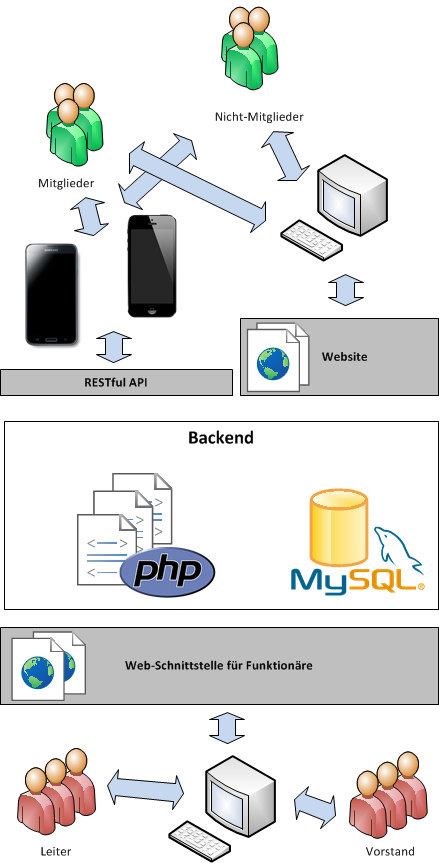
\includegraphics[scale=0.5]{images/visio/SystemScope.png}
\caption{System Übersicht}
\label{fig:system_scope}
\end{figure}

\section{Backend}\label{arch_backend}
Im \glossarmark{PHP} Backend wird seit diesem Projekt Doctrine (siehe \cite{doctrine} und \cite{dunglas2013persistence}) für das \glossarmark{Object-relational mapping} (\glossarmark{ORM}) verwendet. \glossarmark{ORM} hat den Vorteil, dass in einer Konfiguration Tabellen mit Objekten verknüpft werden können und somit viel Aufwand im Bezug auf die Datenbankkommunikation entfällt. Ein Nachteil bei \glossarmark{ORM} kann sein, dass Funktionen, welche Datenbank spezifisch sind, nicht oder nur mit grossem Aufwand verwendet werden können. Doctrine bietet auch Locking-Mechanismen, welche in diesem Projekt benötigt werden. Es gibt die Möglichkeit die \glossarmark{Entity}-Konfiguration in ein File auszulagern oder mit Annotationen direkt im Objekt zu erfassen, letzteres ist in diesem Projekt der Fall. 

\subsection{Locking}
Das Problem einer Fahrgemeinschaftsverwaltung ist, dass nur eine beschränkte Anzahl an Plätzen zur Verfügung steht. Wenn beispielsweise davon ausgegangen wird, dass es noch drei freie Plätze gibt und vier Mitglieder gleichzeitig auf den Anmelde-Knopf klicken, wäre die Fahrgemeinschaft plötzlich überbucht. Das Szenario ist etwas unwahrscheinlich, die Fahrgemeinschaften werden jedoch immer sehr zeitnah zur Veranstaltung erstellt und somit ist die Zeitspanne, in der sich Mitglieder anmelden, nicht sehr gross. Eine überbuchte Fahrgemeinschaft würde zu Ärger führen, welcher durch ein gezieltes Locking mit wenig Aufwand vermieden werden kann.\\

Es gibt zwei verschiedene Varianten von Locking, das optimistische Locking und das pessimistische Locking. Das optimistische Locking funktioniert indem eine Zeitstempel oder eine Versionsnummer\footnote{Das Verwenden einer Versionsnummer ist oft die bessere Variante, da ein Zeitstempel bei sehr schnellen und hochfrequenten Transaktionen und je nach Auflösungsgenauigkeit Fehler verursachen könnte} angepasst wird, wenn das Objekt verändert wurde. Wenn etwas verändert werden soll, wird diese Versionsnummer mitgeführt und vor dem Speichern geprüft, ob sich die Version seit diesem Zeitpunkt bereits verändert hat. Das pessimistische Locking wird mittels eines Locks, sei es eines zeilen- oder tabellenbasierten, und einer Transaktion durchgeführt.\\

Die Implementation in diesem Projekt sieht für den User wie ein optimstisches Locking aus, alle vier Mitglieder aus dem Beispiel oben sehen den Anmelde-Knopf, lediglich einer erhält am Schluss die Fehlermeldung, dass es keinen Platz mehr hat. Im Backend ist es jedoch mit einem pessimistischen Locking auf Zeilenebene gelöst. Die Transaktion wird eröffnet, die Zeile wird gelockt, der Request wird überprüft, der Eintrag wird gespeichert und danach wird die Zeile mit dem Beenden der Transaktion wieder freigegeben. Um diesen Vorgang etwas besser zu veranschaulichen wurde ein Sequenzdiagramm (siehe Abbildung \ref{fig:locking_verfahren}) erstellt, dies wurde anhand der Vorlage in \cite{soft_arch_book} realisiert.

\begin{figure}[h]
\centering
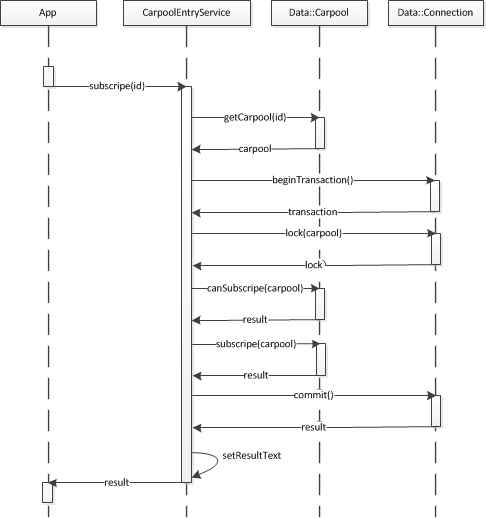
\includegraphics[scale=0.75]{images/visio/locking_verfahren.png}
\caption{Sequenzdiagramm - Locking Verfahren}
\label{fig:locking_verfahren}
\end{figure}

\FloatBarrier
\subsection{API}
Die App enthält so gut wie keine Daten, sondern ruft diese immer direkt vom Backend ab. Dazu wurde ein \glossarmark{RESTful} \glossarmark{API} erstellt, welches \glossarmark{JavaScript Object Notation}-Objekte (\glossarmark{JSON}-Objekte) zurück liefert. Das \glossarmark{API} funktioniert nach dem De-facto-Standard (siehe \cite{wiki_restful}). Bei einem Listen-Aufruf ohne Einträge liefert es eine leere Liste zurück, wenn ein spezifisches Objekt abgerufen wird, liefert es 'null' zurück. Bei Aktionen wird ein \glossarmark{JSON}-Objekt mit den Attributen 'success' und 'error\_message' zurück gegeben.\\

Das \glossarmark{API} hat eine Versionsnummer in der URL, damit kann sichergestellt werden, dass ältere Versionen von der App immer noch lauffähig sind, wenn etwas an der Schnittstelle geändert wird. Dieser Punkt ist sehr wichtig, da man den Usern nicht vorschreiben kann, wann und ob sie ihre App updaten.

\newpage
\section{Lösungsvarianten}\label{loesungsvarianten}
Es gibt verschiedene Wege eine App zu entwickeln und jeder hat seine Vor- und Nachteile. In diesem Abschnitt werden drei verschiedenen Methoden miteinander verglichen und der beste für diesen Anwendungszweck ausgewählt.

\subsection{Native App}\label{architektur_native}
In den Anfängen der App Entwicklung bestand nur diese Variante. Es musste für jede Plattform die bereitgestellte \glossarmark{Integrated Development Environment} (\glossarmark{IDE}) verwendet und die dazugehörige Sprache gelernt werden. Native Apps für Apple iOS nutzen die Programmiersprachen Swift und Objective-C, die mit Hilfe von XCode programmiert werden. Android Apps hingegen werden in Java entwickelt, wofür früher Eclipse Android Development Tools (ADT) und heutzutage Android Studio basierend auf IntelliJ verwendet werden kann. Die Vorteile sind voller Funktionsumfang und gute Unterstützung bei der Entwicklung durch die \glossarmark{IDEs}. Das Verwalten von zwei oder mehreren separaten Code-Sourcen ist jedoch sehr aufwendig.

\subsection{Xamarin}\label{architektur_xamarin}
Xamarin (siehe \cite{xamarin}) ist ein mächtiges Framework, welches es ermöglicht den Code der App in C\# zu schreiben und diesen dann in Native Code umzuwandeln. Xamarin liefert seine eigene \glossarmark{IDE}, kann aber auch in Visual Studio integriert werden. Grosse Firmen wie 3M, AT\&T und HP verwenden Xamarin für ihre Apps. Der grosse Vorteil ist, dass man fast alle Funktionen einer Native App verwenden kann und dazu nur eine Sprache und eine \glossarmark{IDE} beherrschen muss. 

\subsection{Phonegap}\label{architektur_phonegapt}
Phonegap (siehe \cite{phonegap} und \cite{wargo2012phonegap}) basiert auf Cordova (siehe \cite{cordova}), ein Framework von Apache, mit welchem es möglich ist eine in HTML und Javascript geschrieben Webseite in eine Native App umzuwandeln. Phonegap bietet Javascript Plugins, um die Native Funktionen wie zum Beispiel Geolocation, Kompass oder Push-Nachrichten zu benutzen. Das Framework erstellt für die gewünschte Plattform eine App mit einer Webview und fügt die nötigen Klassen für die Plugins hinzu. Ein positiver Nebeneffekt bei dieser Methode ist, dass es möglich ist, die Webseite online zu stellen und alles, ausser den Plugins, zu verwenden. Phonegap bietet im Gegensatz zu den anderen Varianten keine Unterstützung zum Modellieren oder Erstellen grafischer Benutzeroberflächen. Es kümmert sich lediglich um die Konvertierung in die verschiedenen Plattformen und stellt die Schnittstellen zu den Native Funktionen bereit. Phonegap wird oft mit einem für mobile Geräte optimiertem Framework wie zum Beispiel jQuery Mobile (siehe \cite{jquery_mobile} und \cite{reid2011jquery}) kombiniert.

\newpage
\subsection{Nutzwertanalyse}\label{architektur_nutzwertanalyse}

\subsubsection{Bewertungskriterien}\label{architektur_bewertungspunkte}

In der Nutzwertanalyse werden folgende Punkte betrachtet, nach dem angegebenen Schema bewertet und anschliessend gewichtet. Die Kriterien sind grösstenteils aus den Softwarequalitätsmerkmalen nach \cite{iso_9126} abgeleitet.

\paragraph{Aufwand}
\begin{itemize}
	\item \textbf{Beschreibung}: Wie gross ist der geschätzte Aufwand mit dieser Methode?
	\item \textbf{Bewertung}: 1: sehr hoch, 10: sehr niedrig
	\item \textbf{Gewichtung}: 5 (Die Zeit für dieses Projekt ist beschränkt und die Entscheidung könnte zu einem Risiko werden)
\end{itemize}

\paragraph{Benutzbarkeit}
\begin{itemize}
	\item \textbf{Beschreibung}: Wie schnell hat man diese Variante erlernt? 
	\item \textbf{Bewertung}: 1: sehr langsam, 10: sehr schnell
	\item \textbf{Gewichtung}: 4 (Je mehr Zeit für das Erlernen investiert wird, desto weniger Zeit hat man für die Implementierung)
\end{itemize}

\paragraph{Übertragbarkeit}
\begin{itemize}
	\item \textbf{Beschreibung}: Wie flexibel ist diese Variante? Kann sie auf verschiedenen Plattformen laufen? 
	\item \textbf{Bewertung}: 1: sehr spezifisch, nicht portabel, 10: sehr flexibel
	\item \textbf{Gewichtung}: 4 (Die Anforderungen geben vor, dass die App mindestens auf Android und iOS laufen muss)
\end{itemize}

\paragraph{Funktionalität}
\begin{itemize}
	\item \textbf{Beschreibung}: Wie gross ist der Funktionalitätsumfang? 
	\item \textbf{Bewertung}: 1: sehr eingeschränkt, 10: sehr weit reichend
	\item \textbf{Gewichtung}: 3 (In der ersten Version der App wird noch nicht viel Funktionalität gebraucht)
\end{itemize}

\paragraph{Kosten}
\begin{itemize}
	\item \textbf{Beschreibung}: Wie viel kostet diese Lösung? 
	\item \textbf{Bewertung}: 1: sehr teuer, 10: gratis
	\item \textbf{Gewichtung}: 1 (Der Turnverein kommt für die Kosten auf und ist auch bereit etwas dafür zu bezahlen)
\end{itemize}

\newpage
\subsubsection{Bewertung}\label{architektur_bewertung}
Anhand der zuvor definierten Kriterien wurde eine Bewertung vorgenommen. Diese Bewertung ist nicht generell gültig, sie bezieht sich auf die Erfahrung des Entwicklers dieser Arbeit und das Projekt selbst.

\begin{table}[ht]
\centering
  \begin{tabular}{>{\columncolor{darkgray}} l | p{4cm} | p{4cm} | p{4cm}}
	\hline
	\rowcolor{darkgray}
	\textbf{Kriterium}		&	\textbf{Native App}	&	\textbf{Xamarin} 	&	\textbf{Phonegap}	\\ \hline
				&	
\includegraphics{images/icons/ios_android.png}	&	
\includegraphics[scale=0.25]{images/icons/xamarin.png} 	&	
\includegraphics[scale=0.25]{images/icons/phonegap_logo.jpg}	\\ \hline
	\rowcolor{gray}
	\textbf{Aufwand}		&	2 (10)		&	4 (20)		&	7 (35)		\\ \hline
	\textbf{Begründung}		&	Schon beim Support von 2 Plattformen enorm gross	
				&	C\# lernen, in Xamarin einarbeiten			
				&	jQuery Mobile erlernen, Phonegap kennen lernen	\\ \hline
	\rowcolor{gray}
	\textbf{Benutzbarkeit}	&	5 (20)		&	4 (16)		&	7 (28)		\\ \hline
	\textbf{Begründung}		&	Die \glossarmark{IDEs} sind sehr umgänglich, jedoch nicht sehr viel Erfahrung in Objective-C
				&	Keine Erfahrung in C\# und fast keine Erfahrung mit Visual Studio/Xamarin				
				&	Viel Erfahrung in HTML/Javascript, jedoch keine Erfahrung mit jQuery Mobile\\ \hline
	\rowcolor{gray}
	\textbf{Übertragbarkeit}	&	2 (8)		&	7 (28)		&	8 (32)		\\ \hline
	\textbf{Begründung}		&	Jede Plattform benötigt seinen eigenen Code	
				&	Einschränkung bei der Wiederverwendung von UI Code				
				&	Ausser einigen Zeilen exakt der gleiche Code	\\ \hline
	\rowcolor{gray}
	\textbf{Funktionalität}	&	10 (30)	&	9 (27)		&	7 (21)		\\ \hline
	\textbf{Begründung}		&	Alles was die Produkte bieten, kann verwendet werden		
				&	Nahezu alles kann verwendet und gemacht werden				
				&	Plugins bieten nicht den kompletten Funktionsumfang	\\ \hline
	\rowcolor{gray}
	\textbf{Kosten}		&	9 (9)		&	3 (3)		&	9 (9)		\\ \hline
	\textbf{Begründung}		&	Developer Accounts kosten, ansonsten gratis		
				&	Developer Accounts kosten, jedoch Kosten pro Plattform				
				&	Developer Accounts kosten, ansonsten gratis		\\ \hline \hline
	\rowcolor{gray}
	\textbf{Total (gewichtet)}	&	\textbf{28 (77)}	&	\textbf{27 (94)}	&	\textbf{38 (125)}	\\ \hline
  \end{tabular}
   \caption{Nutzwertanalyse - Lösungsvarianten}\label{table:bewertungskriterien}
\end{table}

\FloatBarrier
\subsubsection{Fazit}\label{architektur_fazit}
Das Resultat der Nutzwertanalyse ist eindeutig, die Entwicklung mittels Phonegap ist für dieses Projekt mit Abstand die beste Lösung. Die Methode besitzt noch weitere Vorteile: Etwa dass der Code nur in eine App verpackt wird und nicht in eine andere Sprache übersetzt werden muss, somit gibt es viel weniger Overhead. Zudem ist es, sollte beispielsweise der Support für den Converter eingestellt werden, weiterhin möglich den Quellcode direkt in der Native App anzupassen.

\newpage
\section{Mobile App}\label{moblie_app}

Die Nutzwertanalyse \ref{architektur_nutzwertanalyse} hat gezeigt, dass die beste Methode für dieses Projekt das Phonegap Framework ist. Dies wurde im Projekt umgesetzt und mit jQuery Mobile kombiniert. Die Grundidee von jQuery Mobile ist, dass alle Seiten im selben HTML-File gespeichert werden, bietet jedoch auch die Möglichkeit, die Seiten in verschiedene Files aufzuteilen. In diesem Projekt wurde die zweite Variante gewählt, weil damit die HTML-Files übersichtlich bleiben. Die einzelnen Seiten sind sehr einfach aufgebaut. Sie bestehen aus einer Kopfzeile, in welchem das Menü und die Einstellungen aufgerufen werden können, sowie dem Inhalt, welcher in einer Liste angezeigt wird. Bei Unterseiten wird anstatt dem Menü eine Back-Taste eingeblendet. Die Daten werden über einen jeweiligen \glossarmark{Asynchronous JavaScript and XML}-Request (\glossarmark{Ajax}-Request) vom Backend abgeholt und dann in die ListView abgefüllt.\\

Von Phonegap wurden die Plugins PushNotification, für das Empfangen von Push-Nachrichten, das Device Plugin, sowie das Network-Information Plugin verwendet. Das PushNotification Plugin muss für Android und iOS spezifisch initialisiert werden und um herauszufinden, auf welcher Plattform die App läuft, wurde das Device Plugin verwendet. Das Network-Information Plugin wurde für die Kontrolle der Internetverbindung eingesetzt.\\



